% Source - https://tex.stackexchange.com/a/729099

\documentclass[tikz]{standalone}
\usetikzlibrary{backgrounds,nfold,intersections, spath3}
\makeatletter
\tikzset{offset/.code=\pgfgetpath\tikz@temp\pgfsetpath\pgfutil@empty\pgfoffsetpath\tikz@temp{#1}}
\makeatother
\begin{document}
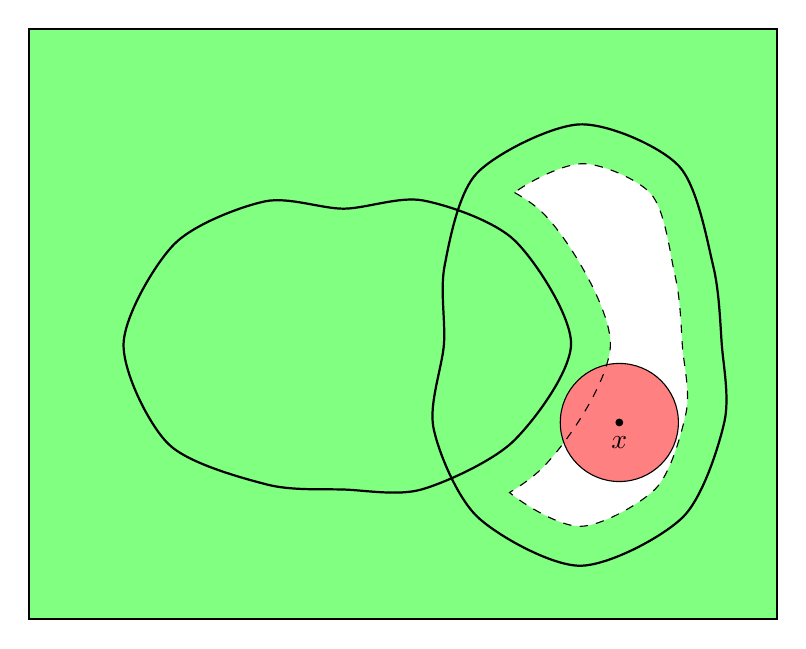
\begin{tikzpicture}[declare function={rrnd(\x)=2.2+0.2*rnd+0.5*cos(2*\x);}]
\pgfmathsetseed{137}
\draw [thick] (-4, -3.5) coordinate (tl) rectangle (5.5,4) coordinate (tr);
\draw [spath/save=random1, thick]
  plot[smooth cycle, samples at={0,30,...,330}] (\x:{rrnd(\x)});
\draw [spath/save=random2, thick, rotate=90, shift={(0,-3)}]
  plot[smooth cycle, samples at={0,30,...,330}] (\x:{rrnd(\x)});
\draw [fill=red!50] (3.5,-1)
  node[fill=black, circle, inner sep=1pt, label=below:{$x$}] {}
  circle[radius=0.75];

\tikzset{
  spath/split at intersections={random1}{random2},
  spath/remove components={random1}{1,3},
  spath/remove components={random2}{1}}
\path[spath/use={random1, reverse}, offset=5mm, spath/save=random1];
\path[spath/use={random2},          offset=5mm, spath/save=random2];
\draw[
  dashed,
  spath/split at intersections={random1}{random2},
  spath/remove components={random1}{1,3},
  spath/remove components={random2}{1,3},
  spath/use={random1},
  spath/use={random2, weld},
  spath/close,
  spath/save=area,
];
\scoped[on background layer]
  \fill[green!50] (tl) rectangle (tr) [spath/use=area];
\end{tikzpicture}
\end{document}
